
\section{Preliminaries} \label{sec:preliminaries}
We first introduce key concepts and notations for our task.

\textbf{Knowledge Graph (KG)}. A KG is a collection of factual knowledge organized in form of triples: $\mathcal{G} =  \{(h,r,t)\} \subseteq \mathcal{E} \times \mathcal{R} \times  \mathcal{E} $, where $\mathcal{E}$ represents the entity set and $\mathcal{R}$ represents relation set. Each triple consists of three elements: a head entity $h$, a relation $r$, and a tail entity or a literal $t$.

\textbf{Logical Form}. The logical form is a structured language representation of a question. In this work, we adopt S-expression $\mathcal{F}$ as our chosen logical expression, following \cite{chatkbqa,decaf}. As shown in the examples provided in Figure \ref{fig:intro}, the S-expression utilizes functions (such as \textit{JOIN}, \textit{AND}) that operate on set-based semantics, which keep a balance between readability and compactness and thus is well-suited for KGQA \cite{gu2021beyond}.

\textbf{KGQA with LLM}. KGQA is a classical NLP task that has been further enhanced through the utilization of LLMs.
Given a question $q$, this task aims to retrieve knowledge related to $q$ from a KG $\mathcal{G}$ and generate an S-expression $\mathcal{F}$. Since many KG storage engines support SPARQL, the generated S-expression $\mathcal{F}$ is converted into a SPARQL query, which is further executed against $\mathcal{G}$ to obtain the final answers. In our work, We retrieve multi-aspect knowledge (including entities $k_e$, relations $k_r$, and subgraphs $k_s$) and design a model $f$ that utilizes LLMs to generate $\mathcal{F}$ based on question and retrieval knowledge as input, i.e., $\mathcal{F} = f(q,k_e,k_r,k_s)$. By converting and executing the SPARQL query on the KG, we can obtain final answers denoted as $a = query(convert(\mathcal{F})) \in \mathcal{A}_q$, where $\mathcal{A}_q \subseteq \mathcal{E}$.


\section{Methodology} \label{sec:method}
In this section, as shown in Figure \ref{fig:method}, we begin with multi-aspect knowledge retrieval. We then delve into two specific modules, providing detailed explanations of their functionalities, and demonstrate the process of querying KG using logical form.
\begin{figure*}[t]
\centering
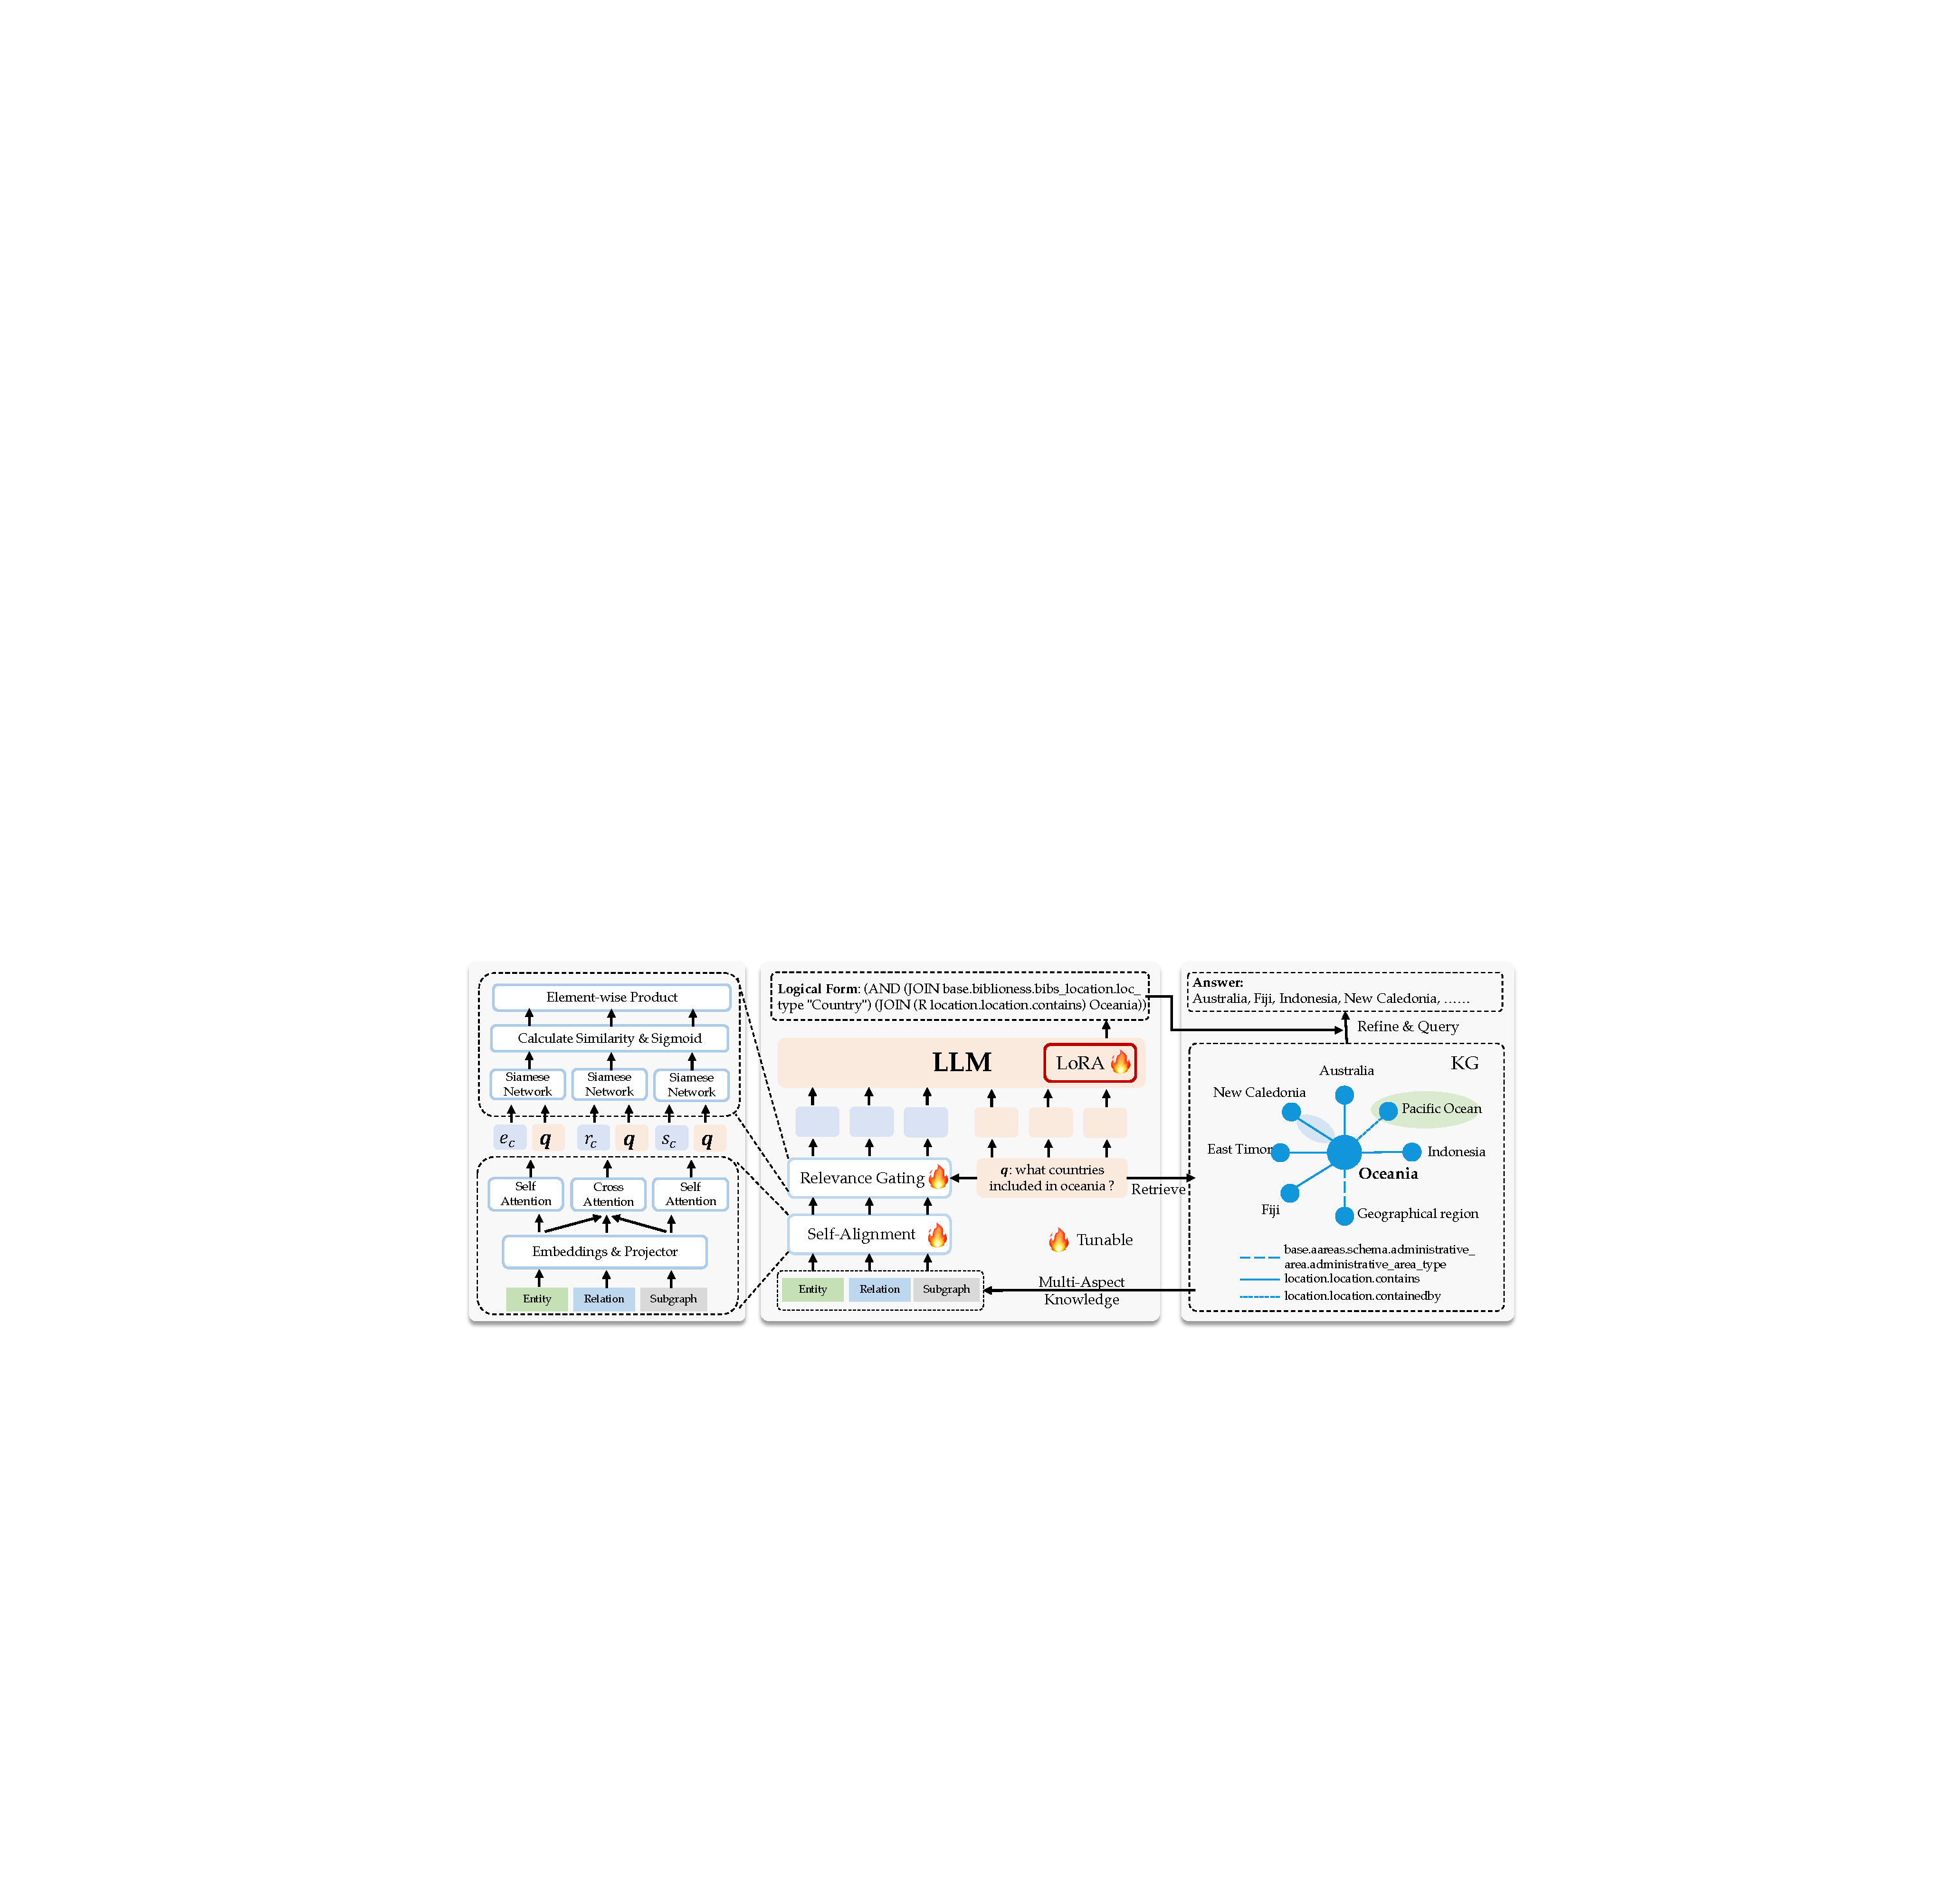
\includegraphics[width=0.9\linewidth]{img/method.pdf}
\caption{Overall framework of \model. We retrieve multi-aspect knowledge from KG and obtain weighted consistency prompt embeddings using Self-Alignment and Relevance Gating modules. These embeddings are combined with the question and fed into LLMs. The generated logical expression is refined and used to query KG, ultimately getting final answers. The unlabeled color blocks in the middle represent the tokens input to the LLM, with pink blocks denoting question tokens and blue blocks denoting retrieved knowledge tokens.
}
\label{fig:method}
\end{figure*}

\subsection{Retrieval of Multi-Aspect Knowledge} \label{sec:Retrieve Multi-level Knowledge}
Previous KGQA methods either focus on retrieving entities and relations \cite{GMT-KBQA} or retrieving multiple triplets to form subgraphs \cite{decaf,G-retriever}. 
In our research, we propose to leverage three types of knowledge simultaneously. Each possesses varying aspects of information, which complement each other and also share commonalities. This enables us to effectively align crucial knowledge across three types.
Due to the differences in their representations (e.g., length and format), we employ different retrieval methods for each type.

\textbf{Entity Retrieval.} 
One effective approach for retrieving candidate entities $k_e$ is to conduct entity linking with question $q$. Following \citet{GMT-KBQA}, we employ the ELQ \cite{ELQ} for question entity linking, which utilizes a bi-encoder to simultaneously detect mentions and link them to entities end-to-end. Then FACC1 \cite{facc1} (a comprehensive Freebase annotation of corpora) is employed to identify entities that were not linked by ELQ, to enhance the range of candidate entities.

\textbf{Relation Retrieval.}
In large-scale KG (e.g. Freebase), relations are typically organized hierarchically, such as the example \textit{base.biblioness.bibs\_location.loc\_type}. Therefore, directly using question-based dense retrieval for similarity may not be effective. To address this, following \citet{GMT-KBQA}, we propose masking entity mentions detected during the candidate entity retrieval stage with a [BLANK] token for each question $q$. Building on the work of \citet{GMT-KBQA,CBR-KBQA}, we train two separate BERT models that encode questions and relations into a shared dense space. The objective of optimization is to maximize the score of the relevant relation compared to randomly sampled relations. To retrieve the nearest relations, we employ FAISS \cite{douze2024faiss}, a highly efficient vector database, which allows us to speed up the search process and obtain the most relevant results. 

\textbf{Subgraph Retrieval.}
One crucial consideration is the wealth of structural and semantic information contained within KG. 
Since KG data is typically stored as triplets, we linearize triplets by combining head entity, relation, and tail entity for retrieval. Following \cite{decaf}, we propose grouping linearized sentences with the same head entity into a document. To save computing resources, we only focus on 1-hop subgraphs to capture structural information.
Furthermore, concerning the potential information loss when converting long documents into vectors, we employ sparse retrieval approaches that rely on keyword dependencies. Specifically, we employ techniques like BM25, which calculates TF-IDF scores based on sparse word matches between input questions and KB-linearized passages. For more information, refer to the appendix.


\subsection{Self-Alignment} \label{sec:Self-Alignment}
Although multi-aspect retrieval offers comprehensive auxiliary information, it can also introduce irrelevant knowledge and noise, resulting in negative impacts. To address this concern, we propose to align the commonalities among multi-aspect information to improve informativeness.

We first utilize LLM's embedding layer to convert the multi-aspect retrieval knowledge into text embeddings $\boldsymbol{X}_{e} \in \mathbb{R}^{t_k \times l \times e}$, where the $t_k$ represent top $k$ retrieval texts, $l$ denotes the maximum length of text, and $e$ indicate the embedding dim of the token. We then apply an averaging operation, followed by a projector network \(\mathcal{M}\), which transforms these embeddings into prompt embeddings $\boldsymbol{X}_{t} \in \mathbb{R}^{t_k \times e}$ (\textit{i.e.}, one piece of retrieval text is projected to one token embedding). For the sake of efficiency, $\mathcal{M}$ is designed to consist of down-projection and up-projection layers, with a nonlinear layer situated between them, as follows:

\begin{equation}
\begin{aligned}
    &\boldsymbol{X}_{e} = Embeddings({T}), \\
    &\boldsymbol{X}_{t} = \mathcal{M}(\hat{\boldsymbol{X}}_{e}), \quad \hat{\boldsymbol{X}}_{e} =  \frac{1}{l}\sum\nolimits_{i=1}^{l} \boldsymbol{X}_e[:,i,:],\\
\end{aligned}
\end{equation}
where $T$ represents the retrieval text of entities, relations, or subgraphs.
Next, we apply self-attention separately to the prompt embeddings of entities and relations to obtain entity-consistency tokens $\boldsymbol{e}_{c} $ and relation-consistency tokens $\boldsymbol{r}_{c} $:
\begin{equation}
\begin{aligned}
    &\boldsymbol{e}_{c} = Self\text{-}Attn(\boldsymbol{E}_{t}) \in \mathbb{R}^{t_k \times e}, \\
   &\boldsymbol{r}_{c} = Self\text{-}Attn(\boldsymbol{R}_{t}) \in \mathbb{R}^{t_k \times e}, \\
\end{aligned}
\end{equation}

Here, we use $\boldsymbol{S}_{t}$, $\boldsymbol{E}_{t}$, and $\boldsymbol{R}_{t}$ represent prompt embeddings $\boldsymbol{X}_{t}$ of subgraphs, entities, and relations, respectively.
This attention is applied to individual retrieval text (e.g., one sentence) rather than individual tokens to learn the correlation and consistency between different retrieval information and their importance within the entire top $k$ retrieval data.

In addition, we further focus on leveraging subgraphs information. To determine the significance of retrieval text, we employ entities and relations as alignment factors. As shown in Figure \ref{fig:method}, by aligning triples in a subgraph that is highly consistent to relation  `\textit{location.location.contains}', we can weight important data through commonalities of multi-aspect knowledge. To obtain subgraph-consistency tokens $s_{c}$, we perform cross-attention to entity-subgraph and relation-subgraph pairs, respectively:
\begin{equation}
\begin{aligned}
    &\boldsymbol{s}_{c}^{e} = Cross\text{-}Attn(\boldsymbol{S}_{t}, \boldsymbol{E}_{t} ,\boldsymbol{E}_{t}) \in \mathbb{R}^{t_k \times e}, \\
   &\boldsymbol{s}_{c}^{r} = Cross\text{-}Attn(\boldsymbol{S}_{t}, \boldsymbol{R}_{t} ,\boldsymbol{R}_{t}) \in \mathbb{R}^{t_k \times e}, \\
\end{aligned}
\end{equation}
and sum the results to get $\boldsymbol{s}_{c}= \boldsymbol{s}_{c}^{e} + \boldsymbol{s}_{c}^{r} \in \mathbb{R}^{t_k \times e}$. The consistency tokens of entity $\boldsymbol{e}_{c}$, relation $\boldsymbol{r}_{c}$, and subgraph $\boldsymbol{s}_{c}$ contain refined knowledge aligned between multi-aspect information, enhancing the utilization of the retrieved data.

\subsection{Relevance Gating} \label{sec:Relevance Gating}
After obtaining the consistency tokens, we expect the model to learn the relevance between retrieval data and the question.  The relevance is used to construct a soft gating mechanism, which will adaptively select the relevant retrieval information to be utilized.
To achieve this, we design a siamese network for each type of consistency token to measure its relevance to the question embedding $\boldsymbol{Q}_{e} \in \mathbb{R}^{l \times e}$. Each siamese network consists of a shared MLP $\mathcal{M}_{share}$ networks that processes both question embedding and consistency tokens, the generated $\boldsymbol{q}_{m}\in \mathbb{R}^{l \times e}$ and $\boldsymbol{x}_{c}\in \mathbb{R}^{t_k \times e}$ are then used to calculate similarity score $\boldsymbol{G}_{sim} \in \mathbb{R}^{t_k \times l}$ through a batch matrix multiplication. This score is subsequently averaged, and a sigmoid activation function is applied to produce the final relevance score $\boldsymbol{g}$, as described below:
\begin{equation}
\begin{aligned}
    &\boldsymbol{q}_{m} = \mathcal{M}_{share}(\boldsymbol{Q}_{e}), \quad \boldsymbol{x}_{c} = \mathcal{M}_{share}(\boldsymbol{X}_{c}), \\
    & \boldsymbol{g} = Sigmoid(\frac{1}{l}\sum\nolimits_{i=1}^{l} \boldsymbol{G}_{sim}[:,i]),\quad \boldsymbol{G}_{sim} = \boldsymbol{x}_{c} \cdot  \boldsymbol{q}_{m}^T.\\
\end{aligned}
\end{equation}

Here $\boldsymbol{X}_{c}$ can be denoted as entities, relations, or subgraphs consistency tokens.
The relevance score of entity $\boldsymbol{g}_{e}$, relations $\boldsymbol{g}_{r}$ and subgraph $\boldsymbol{g}_{s}$ serve as soft gates, are used to model the influence of each consistency tokens by element-wise product, respectively:
\begin{equation}
\begin{aligned}
&\boldsymbol{e}_{c}^{w} = \boldsymbol{g}_{e}\circ \boldsymbol{e}_{c}, 
&\boldsymbol{r}_{c}^{w} = \boldsymbol{g}_{r}\circ \boldsymbol{r}_{c},  \quad
&\boldsymbol{s}_{c}^{w} = \boldsymbol{g}_{s}\circ \boldsymbol{s}_{c}.
\end{aligned}
\end{equation}

To enhance generalization ability, we introduce randomly initialized soft tokens $\boldsymbol{p} \in \mathbb{R}^{l \times e}$, which are concatenated with the weighted consistency tokens and the question embedding. These combined embeddings are then fed into LLMs to generate logical form $\mathcal{F}$ as follows:

\begin{equation}
 % \mathcal{F} = \prod \limits_{i=1}^r p_{\theta,\phi_1,\phi_2}(y_i|y_{<i},[{e}_{c}^{w};{r}_{c}^{w};{s}_{c}^{w};{Q}_{e}]),
 \mathcal{F} = f_{\theta,\phi_1,\phi_2}([\boldsymbol{p};\boldsymbol{e}_{c}^{w};\boldsymbol{r}_{c}^{w};\boldsymbol{s}_{c}^{w};\boldsymbol{Q}_{e}]),
\end{equation}
where [;] represents concatenation operation, the parameters $\theta$ of LLMs itself are frozen. The parameters that require back-propagation optimization include our model parameters $\phi_1$ and LoRA parameters $\phi_2$.


\subsection{Query Execution} \label{sec:Query Execution}
Due to the long-tail distribution of fine-tuned data and the lack of specific knowledge, LLM may not strictly adhere to the contextual information provided \cite{chatkbqa}. As a result, the generated logical forms may contain non-existent entities or relations. For instance, when asked `\textit{where was rihanna born and raised?}', an LLM might generate the logical form `\textit{(JOIN (R people.person.place\_of\_birth) Rihana)}' instead of the correct spelling `\textit{Rihanna}'. This discrepancy renders the logical form non-executable on KG, and the same issue can also arise with relations.

To further refine the quality of entity and relation, we employ a similarity-based approach with KG. Specifically, we utilize an unsupervised SimCSE model to measure the similarity between each entity in the generated logical form $\mathcal{F}$ and the labels of entities in the entity set $\mathcal{E}$. By setting a threshold, we retain the most relevant entities $\mathcal{E}_{sub}$. Additionally, we query the KG to identify relations $\mathcal{R}_{2-hop}$ that are within 2 hops of the obtained subset of entities $\mathcal{E}_{sub}$. Similarly, we calculate the similarity between all relations in $\mathcal{F}$ and the identified set of relations. This refinement process allows us to generate a new list of candidate logical forms $\mathcal{F}_{new}$ that better align with the KG. After converting to SPARQL language, it can be used to query answers from KG: $a = query(convert(\mathcal{F}_{new}))$. 

